\chapter{Implementation}

TODO: Chapter introduction

\textbf{COMMENT: Perhaps upfront explain the process with the prototypes?}

\section{Proof of Concept}
Before the actual implementation of the design from the previous Chapter, a Proof of Concept (PoC) was created. This had several purposed, first to see if it was at all possible to have at least some sense of the scale when performing the gestures, secondly \textbf{?? what are other good reasons?}. The component listed bellow was connected together as shown in Figure \ref{sketch_bb} and \ref{sketch_schem}, the finished PoC can be seen in Figure \ref{poc}. The 

\begin{itemize}
    \item Adafruit Feather M0 Adalogger\cite{adalogger} with a 340mAh 3.7V battery
    \item Adafruit 9-DOF Absolute Orientation IMU Fusion Breakout - BNO055\cite{gyro}
	\item Flora Wearable Bluefruit LE Module\cite{bluefruit}
	\item A push button
	\item A 100k$\Omega$ resistor
\end{itemize}

\begin{figure}[h!]
    \centering
    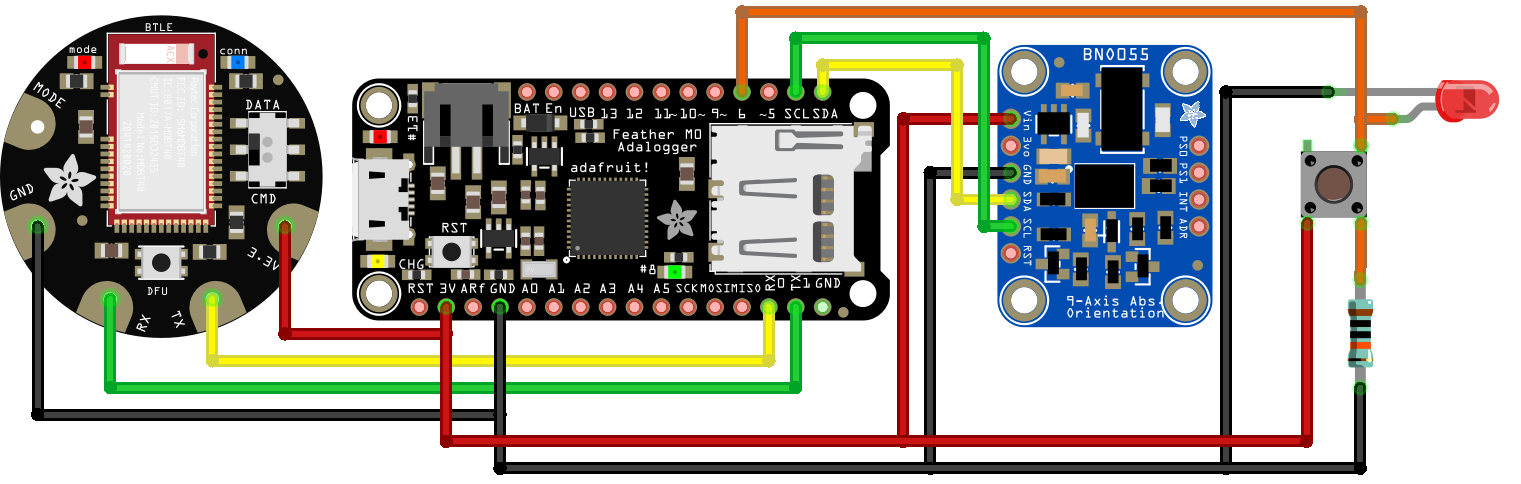
\includegraphics[width=1\textwidth]{figures/Sketch_bb.png}
    \caption{Wiring for of the proof of concept. Battery not shown}
    \label{sketch_bb}
\end{figure}

\begin{figure}[h!]
    \centering
    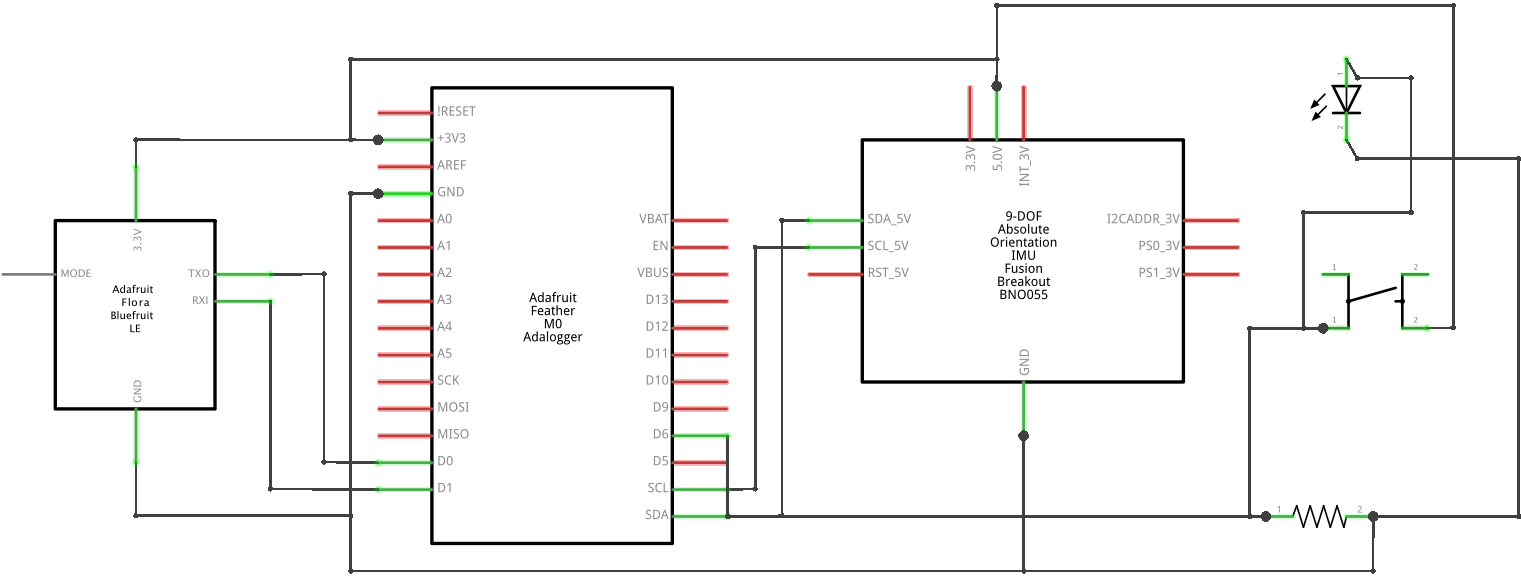
\includegraphics[width=1\textwidth]{figures/Sketch_schem.png}
    \caption{Schematic for the proof of concept. Battery not shown}
    \label{sketch_schem}
\end{figure}

\begin{figure}[h!]
    \centering
    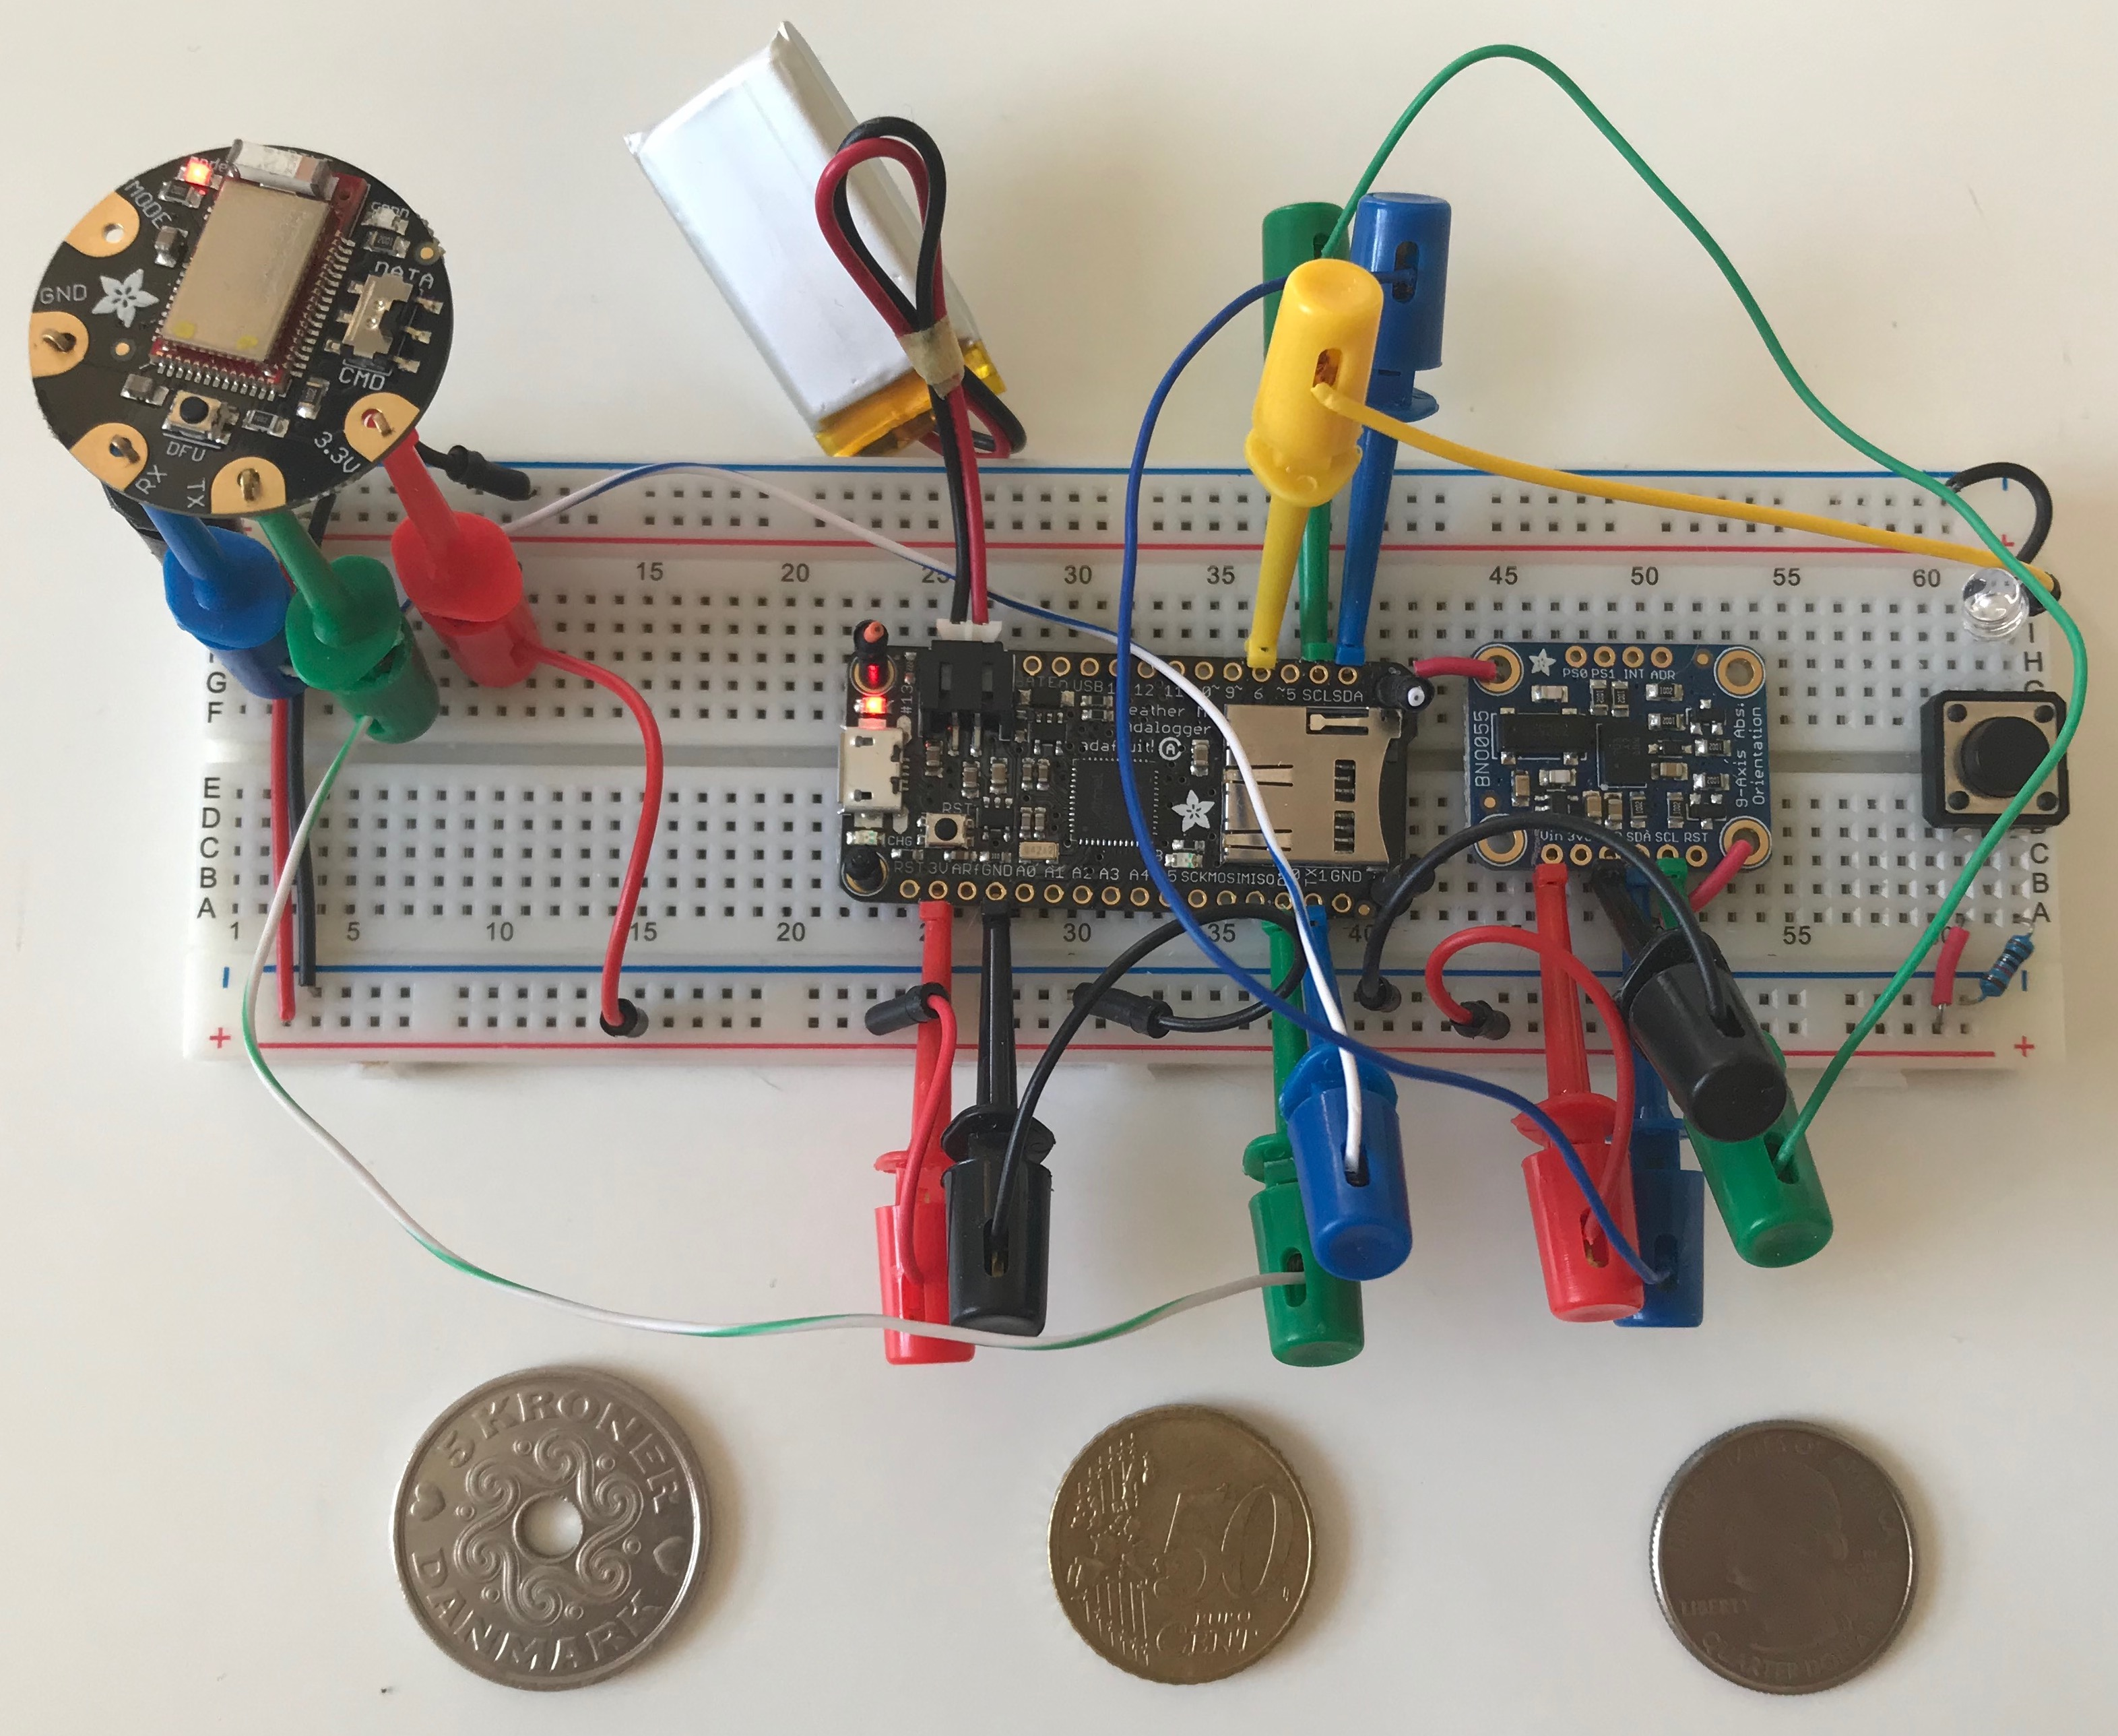
\includegraphics[width=1\textwidth]{figures/poc.jpg}
    \caption{Proof of concept. Components from left to right on the breadboard: Bluefruit LE Module, Feather M0 Adalogger and battery, IMU Fusion Breakout - BNO055, push button and led. Coins below for scale}
    \label{poc}
\end{figure}


\section{Prototype}

\subsection{MetaMotionR}

\section{Android App}

\section{Testing}

